\RequirePackage[l2tabu,orthodox]{nag}

% TODO: decide if one-sided/two-sided
%\documentclass[headsepline,footsepline,footinclude=false,fontsize=11pt,paper=a4,listof=totoc,bibliography=totoc,BCOR=12mm,DIV=12]{scrbook} % two-sided
\documentclass[headsepline,footsepline,footinclude=false,oneside,fontsize=11pt,paper=a4,listof=totoc,bibliography=totoc]{scrbook} % one-sided

% TODO: change citation style in settings
% TODO: Logo on title page
\PassOptionsToPackage{table,svgnames,dvipsnames}{xcolor}

\usepackage[utf8]{inputenc}
\usepackage[T1]{fontenc}
\usepackage[sc]{mathpazo}
\usepackage[ngerman,american]{babel}
\usepackage[autostyle]{csquotes}
\usepackage[%
  backend=biber,
  url=false,
  style=alphabetic,
  maxnames=4,
  minnames=3,
  maxbibnames=99,
  giveninits,
  uniquename=init]{biblatex} % TODO: adapt citation style
\usepackage{graphicx}
\usepackage{scrhack} % necessary for listings package
\usepackage{listings}
\usepackage{lstautogobble}
\usepackage{tikz}
\usepackage{pgfplots}
\usepackage{pgfplotstable}
\usepackage{booktabs}
\usepackage[final]{microtype}
\usepackage{caption}
\usepackage[hidelinks]{hyperref} % hidelinks removes colored boxes around references and links

\bibliography{bibliography}

\setkomafont{disposition}{\normalfont\bfseries} % use serif font for headings
\linespread{1.05} % adjust line spread for mathpazo font

% Add table of contents to PDF bookmarks
\BeforeTOCHead[toc]{{\cleardoublepage\pdfbookmark[0]{\contentsname}{toc}}}

% Define TUM corporate design colors
% Taken from http://portal.mytum.de/corporatedesign/index_print/vorlagen/index_farben
\definecolor{TUMBlue}{HTML}{0065BD}
\definecolor{TUMSecondaryBlue}{HTML}{005293}
\definecolor{TUMSecondaryBlue2}{HTML}{003359}
\definecolor{TUMBlack}{HTML}{000000}
\definecolor{TUMWhite}{HTML}{FFFFFF}
\definecolor{TUMDarkGray}{HTML}{333333}
\definecolor{TUMGray}{HTML}{808080}
\definecolor{TUMLightGray}{HTML}{CCCCC6}
\definecolor{TUMAccentGray}{HTML}{DAD7CB}
\definecolor{TUMAccentOrange}{HTML}{E37222}
\definecolor{TUMAccentGreen}{HTML}{A2AD00}
\definecolor{TUMAccentLightBlue}{HTML}{98C6EA}
\definecolor{TUMAccentBlue}{HTML}{64A0C8}

% Settings for pgfplots
\pgfplotsset{compat=newest}
\pgfplotsset{
  % For available color names, see http://www.latextemplates.com/svgnames-colors
  cycle list={TUMBlue\\TUMAccentOrange\\TUMAccentGreen\\TUMSecondaryBlue2\\TUMDarkGray\\},
}

% Settings for lstlistings
\lstset{%
  basicstyle=\ttfamily,
  columns=fullflexible,
  autogobble,
  keywordstyle=\bfseries\color{TUMBlue},
  stringstyle=\color{TUMAccentGreen}
}


\newcommand*{\getUniversity}{Technische Universität München}
\newcommand*{\getFaculty}{Department of Informatics} %TODO Check
\newcommand*{\getTitle}{Transferring Hardware-related Information in sys-sage Across Processes and HPC Nodes}
\newcommand*{\getTitleGer}{Übertragung von Hardware-Informationen in sys-sage Bibliothek Zwischen Prozessen und HPC Knoten}
\newcommand*{\getAuthor}{Finn Romaneessen}
\newcommand*{\getDoctype}{Bachelor's Thesis in Informatics}
\newcommand*{\getSupervisor}{Prof. Dr. Martin Schulz}
\newcommand*{\getAdvisor}{Stepan Vanecek}
\newcommand*{\getSubmissionDate}{May 15th, 2024}
\newcommand*{\getSubmissionLocation}{Munich}

\lstset{language=C++,keywordstyle={\bfseries \color{blue}}}

\begin{document}

\pagenumbering{alph}
\begin{titlepage}
  % HACK for two-sided documents: ignore binding correction for cover page.
  % Adapted from Markus Kohm's KOMA-Script titlepage=firstiscover handling.
  % See http://mirrors.ctan.org/macros/latex/contrib/koma-script/scrkernel-title.dtx,
  % \maketitle macro.
  \oddsidemargin=\evensidemargin\relax
  \textwidth=\dimexpr\paperwidth-2\evensidemargin-2in\relax
  \hsize=\textwidth\relax

  \centering

  \IfFileExists{logos/tum.pdf}{%
    \includegraphics[height=20mm]{logos/tum.pdf}
  }{%
    \vspace*{20mm}
  }

  \vspace{5mm}
  {\huge\MakeUppercase{\getFaculty{}}}\\

  \vspace{5mm}
  {\large\MakeUppercase{\getUniversity{}}}\\

  \vspace{20mm}
  {\Large \getDoctype{}}

  \vspace{15mm}
  {\huge\bfseries \getTitle{}}

  \vspace{15mm}
  {\LARGE \getAuthor{}}

  \IfFileExists{logos/faculty.pdf}{%
    \vfill{}
    \includegraphics[height=20mm]{logos/faculty.pdf}
  }{}
\end{titlepage}


\frontmatter{}

\begin{titlepage}
  \centering

  \IfFileExists{logos/tum.pdf}{%
    \includegraphics[height=20mm]{logos/tum.pdf}
  }{%
    \vspace*{20mm}
  }

  \vspace{5mm}
  {\huge\MakeUppercase{\getFaculty{}}}\\

  \vspace{5mm}
  {\large\MakeUppercase{\getUniversity{}}}\\

  \vspace{20mm}
  {\Large \getDoctype{}}

  \vspace{15mm}
  {\huge\bfseries \getTitle{} \par}

  \vspace{10mm}
  {\huge\bfseries \foreignlanguage{ngerman}{\getTitleGer{}} \par}

  \vspace{15mm}
  \begin{tabular}{l l}
    Author:          & \getAuthor{} \\
    Supervisor:      & \getSupervisor{} \\
    Advisor:         & \getAdvisor{} \\
    Submission Date: & \getSubmissionDate{} \\
  \end{tabular}

  \IfFileExists{logos/faculty.pdf}{%
    \vfill{}
    \includegraphics[height=20mm]{logos/faculty.pdf}
  }{}
\end{titlepage}

\thispagestyle{empty}
\vspace*{0.8\textheight}
\noindent
I confirm that this \MakeLowercase{\getDoctype{}} is my own work and I have documented all sources and material used.

\vspace{15mm}
\noindent
\getSubmissionLocation{}, \getSubmissionDate{} \hspace{50mm} \getAuthor{}

\cleardoublepage{}

\addcontentsline{toc}{chapter}{Acknowledgments}
\thispagestyle{empty}

\vspace*{20mm}

\begin{center}
{\usekomafont{section} Acknowledgments}
\end{center}

\vspace{10mm}

%TODO: Rewrite Acknowledgments
%I extend my sincere gratitude to my advisor, [Advisor's Name], for their invaluable guidance and support throughout my bachelor's thesis.
%Their expertise and encouragement have been pivotal in shaping this research endeavor, and I am deeply grateful for their mentorship.
%Additionally, I would like to thank my professor for graciously allowing me to pursue my thesis at his chair,
%which provided me with a conducive environment for academic exploration and growth.

\cleardoublepage{}

\chapter{\abstractname}

In this thesis, a file backed shared memory system was implemented, which can be used to share \emph{sys-sage} topologies between processes and nodes in HPC systems.
The shared memory regions used to transfer the topologies between the processes are implemented with memory mapped files created using the \lstinline|mmap()| syscall.

To share a \emph{sys-sage} topology, the exporting process recursively copies all components, including attribs and DataPaths, of the chosen topology into the created shared memory region.
Since the virtual memory addresses inside the shared region, all pointers within the topology must be translated to offset based pointers.

All importing processes can then recreate the topology in their local memory, translating the offset based pointers back into regular pointers and recreating the component tree structure.

The performance of the implemented shared memory system is tested using multiple example topologies with different amounts of components, attribs and DataPaths.

Additionally, some limitations of the presented implementation are discussed and suggestions for future improvements are made.
\microtypesetup{protrusion=false}
\tableofcontents{}
\microtypesetup{protrusion=true}

\mainmatter{}

\chapter{Introduction}\label{chapter:introduction}
In high-performance computing (HPC), powerful, highly parallel computers are used to solve various technical challenges in all major scientific areas or any other applications processing
large amounts of data or handling large-scale computations. \cite{hpc_intro}

HPC clusters are complex, heterogeneous systems, consisting of many nodes, each with an ever increasing number of cores.
The hierarchical composition of an HPC systems hardware architecture and its individual components is referred to as hardware \emph{topology}. \cite{topology_intro}

The Message Passing Interface (MPI) is commonly used in HPC systems and other parallel machines to communicate between processes and nodes within the cluster.
This allows each node in a HPC system to execute independent programs in its own local memory, while still cooperating and communicating with the entire cluster as needed. \cite{mpi_intro}

Due to the heterogeneous composition of HPC systems and the high degrees of parallelization utilized,
Non-Uniform Memory Access (NUMA) is often used in HPC clusters to achieve more efficient memory access.
NUMA systems use a distributed memory hierarchy to allow cores faster access to local memory regions, whereas accessing non-local memory can cause severe performance decreases. \cite{nuioa_intro}

As memory bandwidth and cache usage have tremendous impact on the overall performance of highly parallelized HPC systems,
making full use of the hardware topology to schedule processes accordingly is crucial in HPC clusters. \cite{openmp_intro}

Processes working closely together will often benefit from sharing a cache to utilize local memory as much as possible,
whereas independent, memory intensive processes could be better scheduled onto separate processors so as not to limit their memory bandwidth and available cache storage. \cite{hwloc_paper}

Making use of the hardware topology to create an efficient process-mapping has the added advantage of reducing the overall communication costs as related processes will be physically close within the cluster. \cite{topology_intro}

Many tools, such as \emph{Portable Hardware Locality (hwloc)} \cite{hwloc}, already exist to gather information about the hardware topology and make it available for these purposes.
Hwloc is a software library that represents hardware resources such as cores or caches in a hierarchical tree structure
to store easily accessible and versatile information about the hardware topology of HPC systems. \cite{hwloc_paper}

Hwloc collects the entire topology information at startup and makes the static information available to the application. \cite{hwloc_paper}

While this approach offers better performance due to the low overhead at runtime, the topology tree can't be adapted to dynamically changing factors at runtime.

Sys-sage \cite{sys-sage} is a library that extends hwlocs functionality to include dynamically changing hardware information and allow representation of arbitrary custom data.
Since sys-sage is fully compatible with hwloc, users can easily use hwloc to initialize their topology data and complement it with custom data as needed.

\section{Motivation}
As mentioned above, using accurate and current information on the hardware topology of a HPC system
has many applications in optimizing the overall performance of individual programs within the cluster.

Creating a detailed topology in sys-sage can cost significant resources during setup, as many custom attributes, components and DataPaths might need to be created.

Since the hardware topologies of different processes within a node are usually very similar
and different nodes within a cluster often have significant overlap in their topologies as well, creating new topologies in each process and node would cause unnecessary overhead.

Instead, sharing entire topologies or specific component subtrees across processes and nodes of HPC systems could be used to reduce redundant creations of sys-sage topologies.

The objective of this thesis is to add a file backed shared memory implementation to sys-sage, which allows user to share entire topologies or select subtrees with other processes or nodes.

\section{Related Work}\label{section:related_work}
Sharing data between processes and nodes using memory mapped files is not a new concept. In fact, it is widely used across many different sectors many different applications and sectors such as
database management systems and data mining. \cite{crotty22-mmap} \cite{mmap_related_work}

This section highlights different approaches to sharing large amounts of data between processes and nodes using memory mapped files as implemented by different libraries.

\subsection*{hwloc}
As mentioned above, portable hardware locality (hwloc) is the software library on which sys-sage bases its functionality and use cases.
Much like sys-sage, hwloc is used to manage information about a systems hardware topology to improve the performance of HPC clusters.

Hwloc offers users the option to share topologies between processes. To do this, the exporting process must use the \lstinline|hwloc_shmem_topology_write()| function,
which copies the topology into a previously created memory mapped file. The duplicated topology can then be \emph{adopted} by importing processes using \lstinline|hwloc_shmem_topology_adopt()|.
The user can then use the adopted topology as usual, however, it can not be modified anymore. \cite{hwloc_docs}

The hwloc shared memory implementation uses file backed memory mappings with identical virtual memory addresses in each process.
To achieve this, hwloc requires the user to find a memory region of sufficient size that is available in all processes.

This approach has the advantage that pointers inside the memory mapped region will work as usual,
which means the shared topology can be used directly from within the shared memory section without having to be copied into the local memory of importing processes.

On the other hand, this approach puts more responsibility and effort on the users side, as finding a sufficiently large memory region might be difficult to achieve.
Additionally, at the time of exporting the topology, it might not be fully known which processes will be adopting the shared topology during its lifetime, so the chosen memory section might not be available in
all importing processes, which can cause expensive reallocations.

While this approach works well for hwloc, as topologies are mostly static in nature, the more dynamic needs of sys-sage topologies call for a shared memory solution that allows importing processes to change the topology as needed.

\subsection*{sharedstructures}

\emph{Sharedstructures} \cite{sharedstructures} is a small software library available in C++ and Python that can be used to store generic data structures
such as hash tables or queues in file backed shared memory regions.

Contrary to hwlocs implementation, sharedstructures uses offset based pointers within the shared memory region,
as the memory sections are resizable and thus might move during their lifetimes.

Sharedstructures provides custom allocators to manage the data structures in the shared memory region.
These allocators are used to reserve memory space within the shared region and can be chosen based on the memory usage profile of the program.

%\chapter{Related Work}\label{chapter:related_work}

\chapter{Sys-Sage}\label{chapter:sys_sage}
Sys-sage is a software library created to collect, represent and provide data on the hardware topology of HPC systems.
It is designed to extend on the existing hwloc library and provide a more versatile and dynamic use-case.

Since a lot of the hardware related data necessary for complex tasks such as thread scheduling or memory management dynamically changes during the execution of
HPC computations, the hwloc approach of providing static topology information collected on startup is often not sufficient.
Gathering the entire dataset at startup makes it difficult to incorporate user-defined data points into the topology and react to the current state of the system
such as measured bandwidth or memory usage.

Sys-sage is designed specifically to enable users to create highly customized and dynamically changeable hardware topologies and build on top of existing hwloc topologies.

\begin{figure}[ht]
    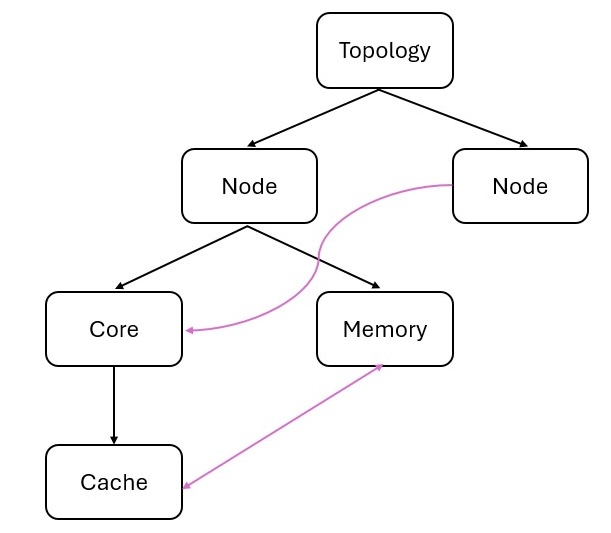
\includegraphics[scale=0.5]{images/Topology_Example.jpg}
    \centering
    \caption{Basic Component Tree with DataPaths}
    \label{figure:topology_example}
\end{figure}

The hierarchical structure of the hardware topology is represented in sys-sage as a tree of \emph{components}.
Each component corresponds to a specific part of the hardware, such as a \emph{cache, core} or \emph{node}.
Depending on the type of component, further information on the underlying hardware can be added to the component, for example the size of a cache.
Additionally, arbitrary attributes can be attached to components to provide further context or add dynamically updated values to the topology. \cite{sys_concept}

Beside the component tree, the \emph{DataPath} graph adds additional information to the topology.
DataPaths are connect two arbitrary components and are used to represent non-hierarchical relationships between components.
Much like components, DataPaths can have custom attributes to add additional data to component relationships. \cite{sys_concept}

\autoref{figure:topology_example} shows a simple example of a topology consisting of two nodes including a few components and DataPaths.
\chapter{Implementation}\label{chapter:Implementation}

The part of the sys-sage library implemented in this thesis enables users to share component subtrees or whole topologies between processes of a compute node by using shared memory regions.

To achieve this, all components of the given subtree, including its attruibutes and all DataPaths, are copied into a memory region shared between the involved processes.
The component tree and DataPath graph are then recreated in the memory of the receiving process.

\section{Capabilities and Usage}
If at any point during the lifetime of a sys-sage topology,

%\section{Limitations}
\section{Shared Memory}
The data sharing aspect of the implementation is realised using shared memory regions. These regions are created by opening files and mapping them using \emph{mmap()}. %TODO code styling?

\emph{mmap()} is a syscall that creates file backed memory mappings in the program's virtual address space that can be opened by multiple processes at once.
The mapped file can then be used just like any regular memory location. \cite{crotty22-mmap}

Using the \emph{MAP\_FIXED} flag when creating a \emph{mmap()} backed memory location will guarantee the virtual memory addresses to be equal across processes.
However, if the necessary memory location is not available in the current process, the mapping will fail, which could potentially have a major impact on the reliability of the library,
depending on the total available memory and its current utilization. [Quote manpage mmap] %TODO

Consequently, the \emph{MAP\_FIXED} flag is not used for the purposes of this thesis to achieve higher reliability when sharing component trees between processes.
As a result, the virtual memory addresses of the shared regions are not identical across processes.

Due to this, sharing pointers to addresses in the shared memory region between processes will not work, as the as the referenced location will have a different address in another process.
Instead, offset based pointers have to be used to reference shared memory locations.

In the sys-sage shared memory implementation, all offsets for pointers are calculated relative to the top of the shared region.
While this might not be possible for more general uses of offset pointers, as the start of the memory location might not always be known,
it is practical for the particular use-case of this thesis, since  memory regions are always handled as a whole and importing only parts of a shared component tree is not supported.

Calculating the offsets based on a shared, fixed location has the advantage that the offset pointers can be used more similarly to regular pointers and don't need to be recalculated when shared.
This means the location of components or DataPaths within the shared memory region can be compared or referenced without amiguity or confusion about the base of the offset.

The lifetime of the shared memory region is handled by a \emph{SharedMemory} object, as shown in \autoref{lst:sharedmemory}.

%TODO Wrap in Figure?
\begin{lstlisting}[language=c++, numbers=left, caption=SharedMemory Class, captionpos=b, label={lst:sharedmemory}]
    class SharedMemory {
      public:
        void* mem;
        char* cur;
        size_t size;
        ...

        SharedMemory(std::string path, size_t size);
        SharedMemory(std::string path);
        ~SharedMemory() { munmap(mem, size); }

      private:
        std::string path;
    };
\end{lstlisting}

Apart from the \emph{path} and \emph{size} size variables, which are used mainly in the creation and destruction of the shared memory region,
the \emph{SharedMemory} class consists of two pointers, \emph{mem} and \emph{cur}.
The \emph{mem} pointer always points to the top of the memory region, whereas the \emph{cur} pointer marks the current location to write or read from while importing or exporting a topology.

When a shared memory region is first created by the process sharing the topology, the path to the file used in the mapping as well as the total size needed have to be known.
The allocated size is then written to the start of the mapped file, to be read by other processes when importing the topology.
The file-backed memory region can then be used to export the topology until the \emph{SharedMemory} destructor is called and the file is unmapped using \emph{munmap()}.

The process importing the topology then uses the constructor in line 9 of \autoref{lst:sharedmemory}, which opens and maps the previously created file,
reads the total size of the data as written by the first process and then remaps the file to that size.
This has the advantage that the total size of the shared topology is always known to the importing process, without having to be provided seperately.
To share a topology, only the path to the memory mapped file needs to be provided, all other information can be read from the file, which simplifies the API and makes it easier
for users to share topologies without much inter-process comunication needed.


[Size Calculation]%TODO

\section{Components}
Topologies consist mainly of \emph{components}, which are organized as a hierarchical tree structure.
Each component represents a certain part of the hardware such as a CPU or cache.

\begin{lstlisting}[language=c++, numbers=left, caption=Component Class, captionpos=b, label={lst:component_class}]
    class Component {
      public:
        map<string,void*> attrib;

      protected:
        int id;
        string name;

        const int componentType;
        vector<Component*> children;
        Component* parent { nullptr };
        vector<DataPath*> dp_incoming;
        vector<DataPath*> dp_outgoing;
    };
\end{lstlisting}

\appendix{}

\microtypesetup{protrusion=false}
\listoffigures{}
\listoftables{}
\microtypesetup{protrusion=true}
\printbibliography{}

\end{document}
